\chapter{Methodology}
%\label{ch:method}


\section{CLANN}
\subsection{Definition}
CLANN (Controlled Language for ANNotation)\footnote{In this document \textit{CLANN} refers to the annotation software platform as well as the grammar} builds on the experiences gained from the previous work, by incorporating redesigned versions of the grammar and the domain ontology.  CLANN is designed to be an end-to-end semantic web application complete with a domain ontology, a persistent layer based on RDF and a user interface for editing and authoring documents.  The domain was expanded to include all the documents in a project specific setting (for example, meeting minutes, status reports, etc).

\subsection{Use case}


\section{PDO Ontology}
%explain the domain of the ontology.
The domain of meeting minutes and status reports was used to engineer an ontology for the purpose of knowledge management.  The initial CLANN prototype was bootstrapped using the the nepomuk ontologies\footnote{\url{www.semanticdesktop.org/ontologies/}} and later extended by the MEMO ontology.  However , the MEMO ontology was only used as a proof of concept implementation of the domain.  Later,  this was completely redesigned and a new ontology PDO (Project Document ontology) was developed in accordance with proper ontology design principles, specifically the Methontology\cite{FLG+97} approach.  The PDO ontology, described using RDFS and OWL-DL, models the inherent structure and concepts of various documents in a project-specific setting, like meeting minutes, status reports etc.   A pictorial representation of the main aspects of the ontology is shown in Figure \ref{figure-pdo}.  \footnote{for a complete specification of the PDO ontology please refer to \url{http://ontologies.smile.deri.ie/pdo} }
% \begin{figure*}
\begin{center}
	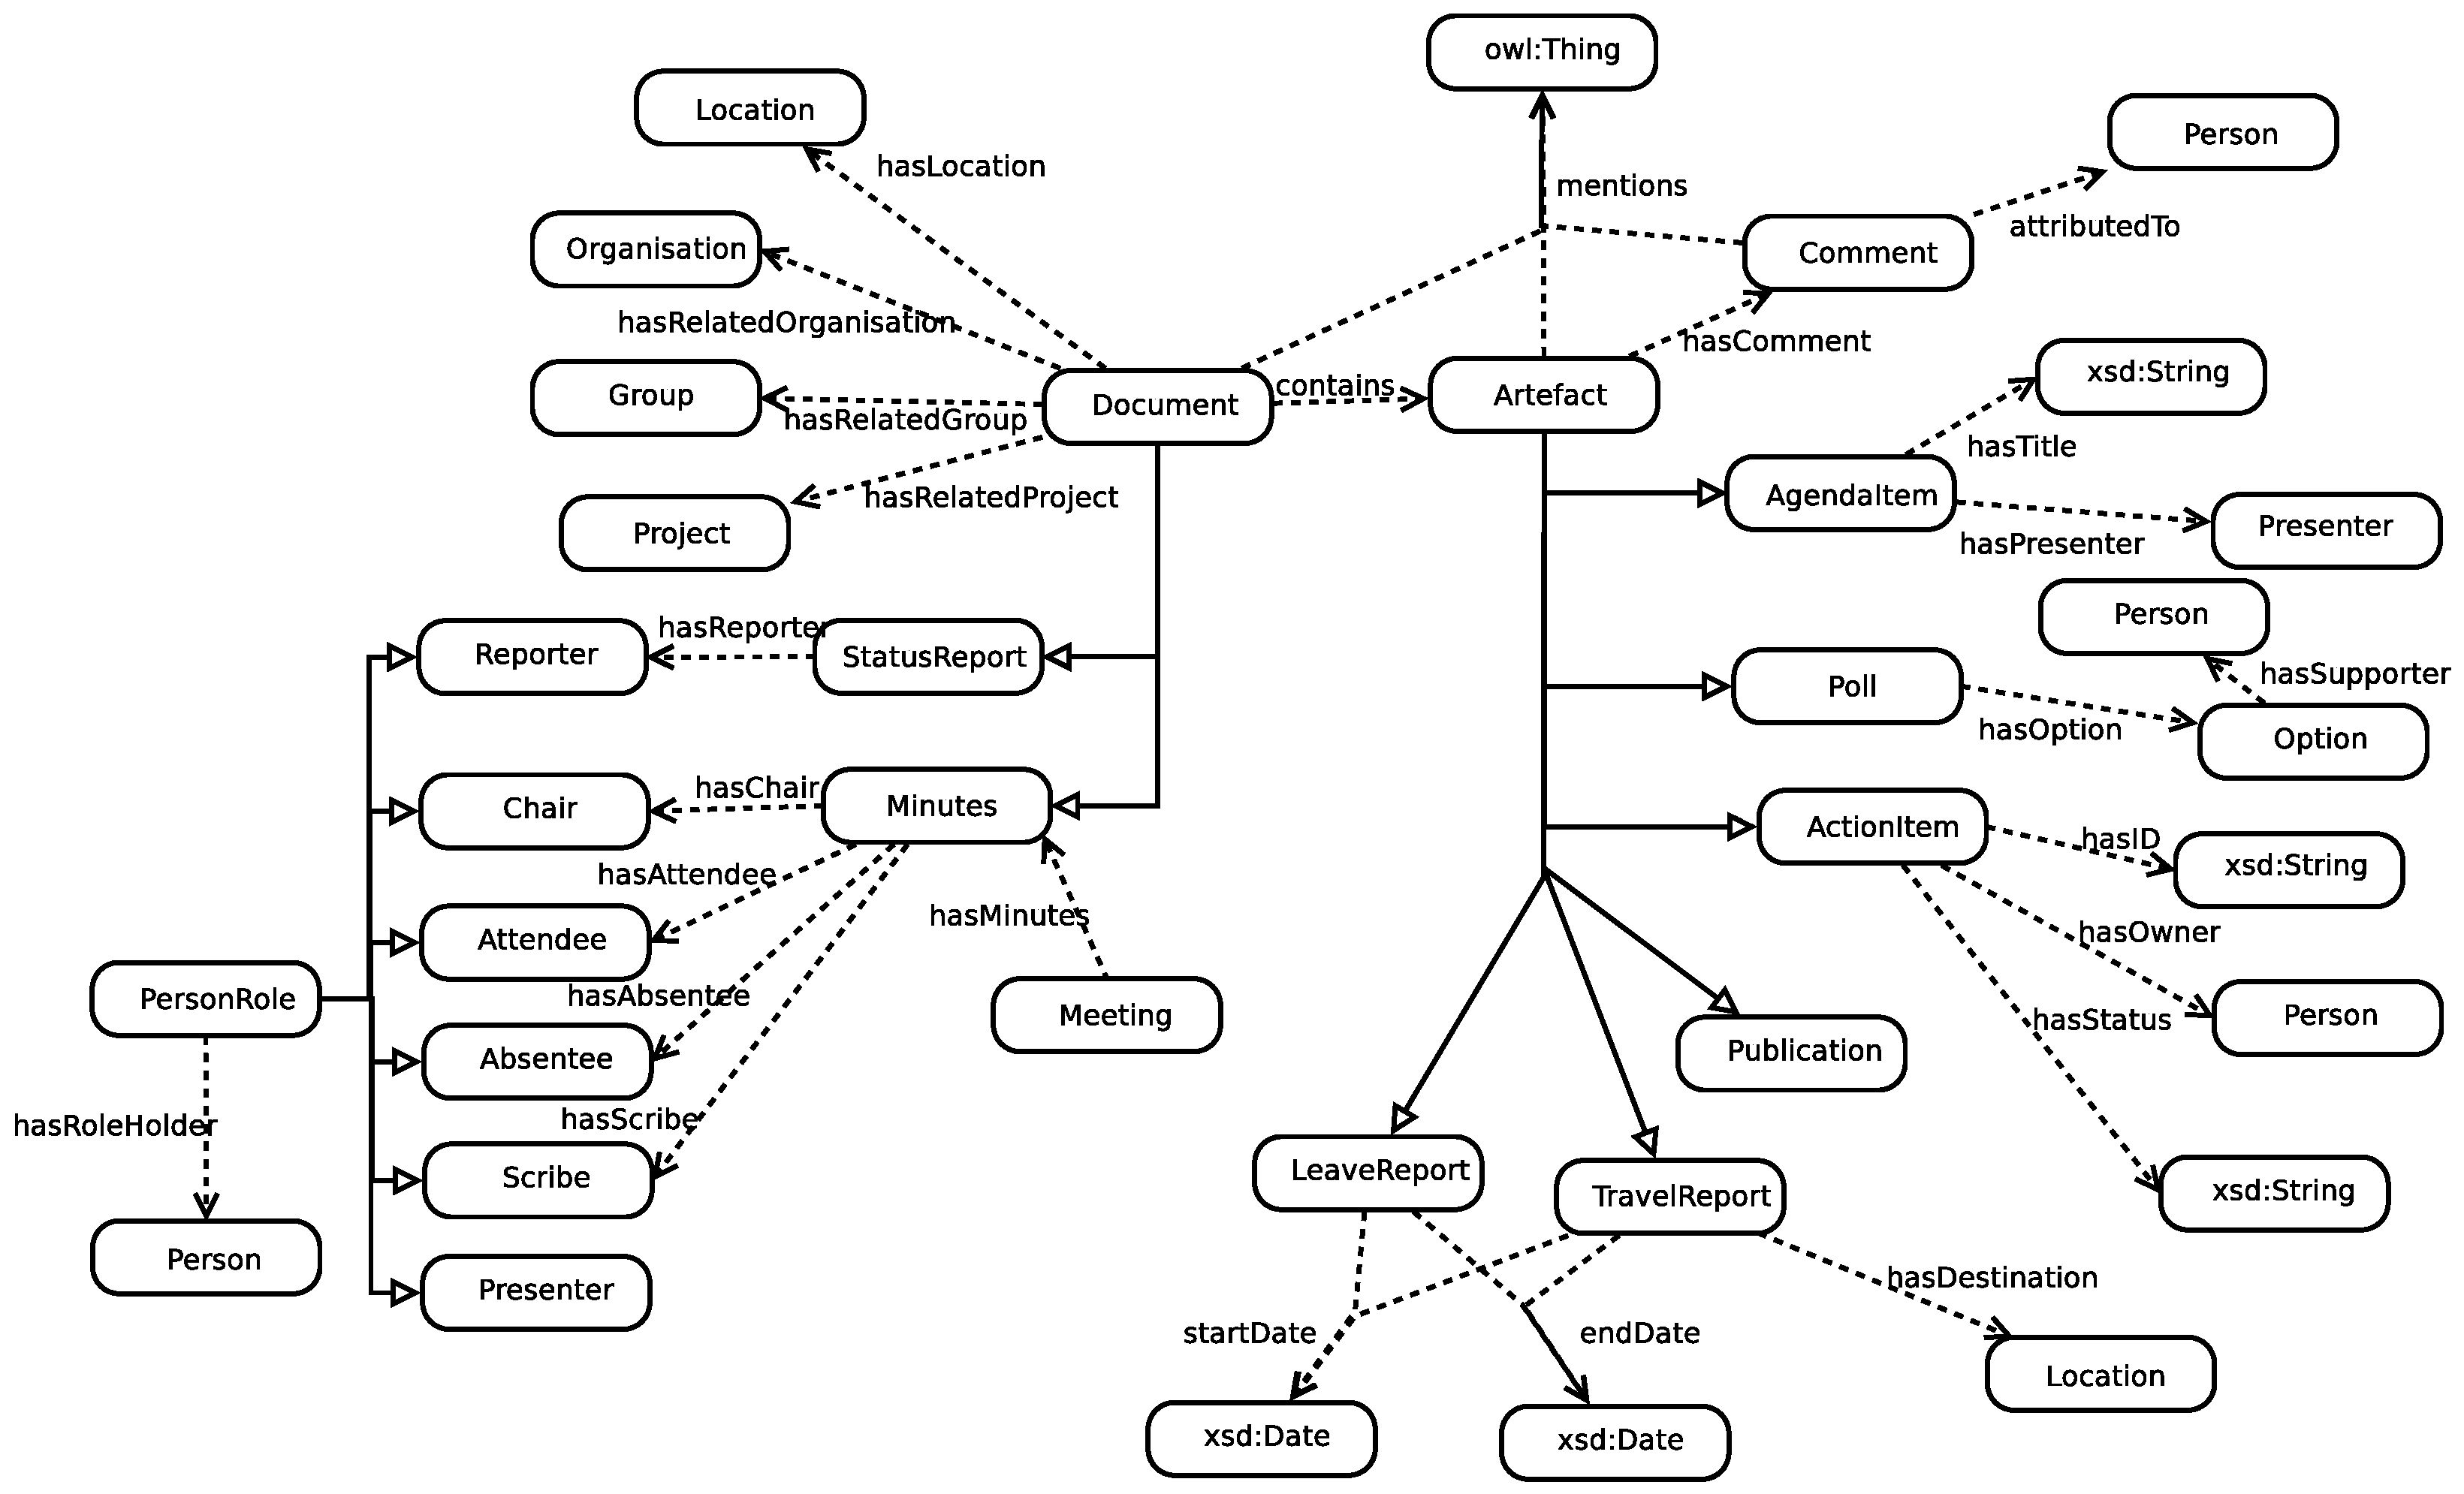
\includegraphics[width=0.8\textwidth]{pdo-v1}
	\caption{Overview of the PDO ontolgoy}
	\label{figure-pdo}
\end{center}
\end{figure*}


\subsection{Design of the ontology}
\subsection{Development and publishing the ontology}


\section{CLANN Grammar}
\subsection{Grammar formalisms}

Various grammar formalisms have been used over the years for understanding natural language.  Phrase structure grammars (PSG), the most widely used formalism, model the inherent structure of the sentences of a language by breaking it into different phrases.  They belong to the class of generative grammars and are composed of a set of productions or rules which break-up the sentences into meaningful phrases.  Dependency grammars(DG), however, concentrate on the links between words without paying attention to the word order.  Structure of a sentence is not broken down into phrases, but determined by adding relations between a head word and its dependent words.  There have been many variations of gramamar formalisms that stemmed out of both PSGs and DGs.  The next few sections describe one such variation of the dependency grammar, the Link grammar, and justifies its selection.

\subsection{Link Grammar}
Link grammars, introduced by \cite{Sleator91}, are a variation of dependency grammars.  Similar to DGs, the link grammars use realtions between words to generate a structure for a sentence.  However, unlike DGs, the links also encode information about directionality and distance.  Moreover, they do not enforce a head-dependent relationship like the DGs.

\cite{Sleator91} defines link grammar as follows:
\begin{quote}\emph{A sequence of words is a sentence of the language if there is a way to draw links between words in such a way that\begin{itemize}
\item the linking requirements of all the words are satisfied,
\item the links do not cross, and
\item the words form a connected graph
\end{itemize} 
}
\end{quote}

The linking requirements of each word are specified as a dictionary, which forms the basis of the link grammar.  Each entry in the dictionary consistes of a word or a group of words belonging to the same grammatical category, appended on the right-hand-side with its linking requirements.  The linking requirements are a series of connectors joined by the logical operators \emph{\&} and \emph{or}.  Each connector denotes the type and direction of the link.  It is a label followed by \emph{+/-} .  \emph{+} denotes a link to the right and \emph{-} denotes a link to the left.  For illustration purposes, an example of a sentence parsed using a very simple link grammar is provided in Figure \ref{figure:link-example}, and an explanation of the same is provided below. 

\begin{figure}[h]
\begin{center}

	\begin{tabular}{l|l}
		\texttt{words} & \texttt{linking requirements}\\
		\hline
		\texttt{the} & \verb#D+#\\
		\texttt{small} & \verb#A+#\\
		\texttt{ate} & \verb#S- & O+#\\
		\texttt{boy apple} & \verb#(A- & D- & S+) or ( D- & O-)#\\
	\end{tabular}
	\begin{verbatim}


 +-----D------+     +----O-----+   
 |     +---A--+--S--+    +--D--+      
 |     |      |     |    |     |              
 the  small  boy   ate  the   apple
\end{verbatim}
	\caption{A sample Link grammar and parse structure.}
	\label{figure:link-example}
\end{center}
\end{figure}



The \emph{D+} connector on the word \emph{the} denotes that \emph{the} is expecting a \emph{D} link to its right.  So It can connect to any word which has a \emph{D-} connector, which, in this case, is either \emph{boy} or \emph{apple}.  The word \emph{ate} has an \emph{\&} operand on \emph{S-} and \emph{O+}.  This means, for the word \emph{ate} to be part of a valid sentence, it should connect to both an \emph{S} connector to its left and an \emph{O} connector to its right.  The case for the nouns \emph{boy} and \emph{apple} is more interesting.  They have two expressions joined by the \emph{or} operand. On closer observation, the first one, \emph{(A- \& D- \& S+)}, models the behavior of a subject noun and the second one, \emph{( D- \& O-)}, models that of an object noun. The reader should also note that the order of the connectors is also valuable. The expression \emph{(A- \& D- \& S+)} also declares the order of linking.  So an \emph{A} link should be made to a word closer than the \emph{D} link. This is illustrated in the parse structure shown in Figure \ref{figure:link-example}. 


\subsection{Why Link Grammar?}

The main design principles for the  CLANN grammar are ease of use and the ability to extend the ontology.  However, the develpoment of the grammar posed different challenges. 

One major priority was to extract RDF tripples from the sentences.  This works very well with the link grammar parse, because the the tripples can directly be extracted by mapping the links.  In the example shown in Figure \ref{figure:link-example}, the tripple \emph{boy ate apple}, can be easily extracted  from the left and right links of the word \emph{ate}.  This is not the case with phrase structure grammars, where extracting dependencies requires detailed ananlysis of the tree structure.   

Another major priority was to develop an intelligent editor on top of the grammar, which supports auto-suggestion and sentence-completion.  An intuitive editor which assists the user while writing the CNL sentences, goes a long way in  helping him to quickly learn the restrictions of the grammar.  This requires an ability to predict text and check the grammatical correctness of partial sentences.  The dictionaries of the link grammar provide valuable information about all the words of the language, which can be exploited for the purpose.
\subsection{Designing the CLANN grammar}
CLANN is designed to enable representing any information that cannot be captured by the templates.  To better explore applicability, two independent prototypes of the grammar CLANN1 and CLANN2 were developed[ref for CNL09]focusing alternatively on usability and expressivity.  This work has eventually led  to CLANN3, which is essentially a merge between the former two grammars, incorporating most of the advantages, albeit a few changes.

\subsubsection{CLANN1 prototype}
CLANN1 is designed with a major focus on usability.  Each sentence adhered to one of the syntactic rules and used a very lenient vocabulary.  This domain vocabulary was derived by corpus analysis using Word Smith tools \footnote{\url{http://www.lexically.net/wordsmith/version5/index.html}} on the document corpus.  This ensured that most of the sentences resembled normal english sentences. CLANN1 is grammatically lax in comparision to typical CNL approaches to knowledge creation. A modified shallow parser is then used to extract the knowledge and instantiate the ontology.
 
\subsubsection{CLANN2 prototype}
CLANN2 was designed with a major focus on expressivity.  It differs from the conventional notion of CNL, whereby the entire document is written in CNL, rather it allows the user to add snippets of CNL text, enclosed in \texttt{"[ ]"}, to the document or associate them to a particular text in the document.These snippets should adhere to a \emph{subject-verb-object} syntax, where the subject is either specified in the snippet or taken from the free text.  The vocabulary for CLANN2 also includes the vocabulary of the ontology, thereby allowing the user to represent any kind of relational meta-data.  This approach was inspired by the CLOnE Language \cite{Funk07}.

The finer details of design and implementation of these grammars are described in \cite{cnl09}.  Both grammars use a common template, described above, which is initially parsed to extract  the inherent meta data of the document (in this case, meeting minutes). 

\subsubsection{CLANN grammar}

 
The CLANN grammar is essentially a combination of CLANN1 and CLANN2, incorporating the snippets of CLANN2 into controlled text of CLANN1 instead of free text.   For other sample documents and information please refer to the project home page\footnote{\url{http://smile.deri.ie/projects/clann}}.


\subsubsection{Templates}
Inorder to supplement the CLANN grammar, we templates which encode implicit domain information, an example of which is shown below.

\begin{minipage}[t]{3.5in}

\texttt{Project Name: <String>\\
Group Name: <String>\\
Date: <Date>\\
Chair: <String>\\
Attendees: (<String>)+\\
Scribe: <String>\\
Action Item:<String>:<String>(:<String>)? (<CNL))+\\
Agenda: <String> (<CNL>)+\\
Poll:<String>:<String> (<String>:<String>)+\\
}
\end{minipage}

These templates were constructed by analysing a collection of in-house meeting minutes and status reports  of the Nepomuk project\footnote{\url{http://dev.nepomuk.semanticdesktop.org/wiki/WikiStart}}.  This approach combines the benefits of the two by using templates for mundane information annotation and CNL for other non-mundane information, consequently minimising the effort and enhancing the user experience.


\section{Design and development of CLANN}
\subsection{CLANN Annotation Platform}
\subsection{Design of the platfrom}
\subsection{Architechture}
\subsection{Modules}
\subsection{Interfaces availiable}
\subsection{Sceenshots}





\subsection{The CLANN grammar}



